%\section{Analysis of the Parameter Space}\label{sec:parameterChoice} 
\section{Setting the RADIUS Parameters}\label{sec:parameterChoice} 

	
\begin{figure*}[t]
	\centering
	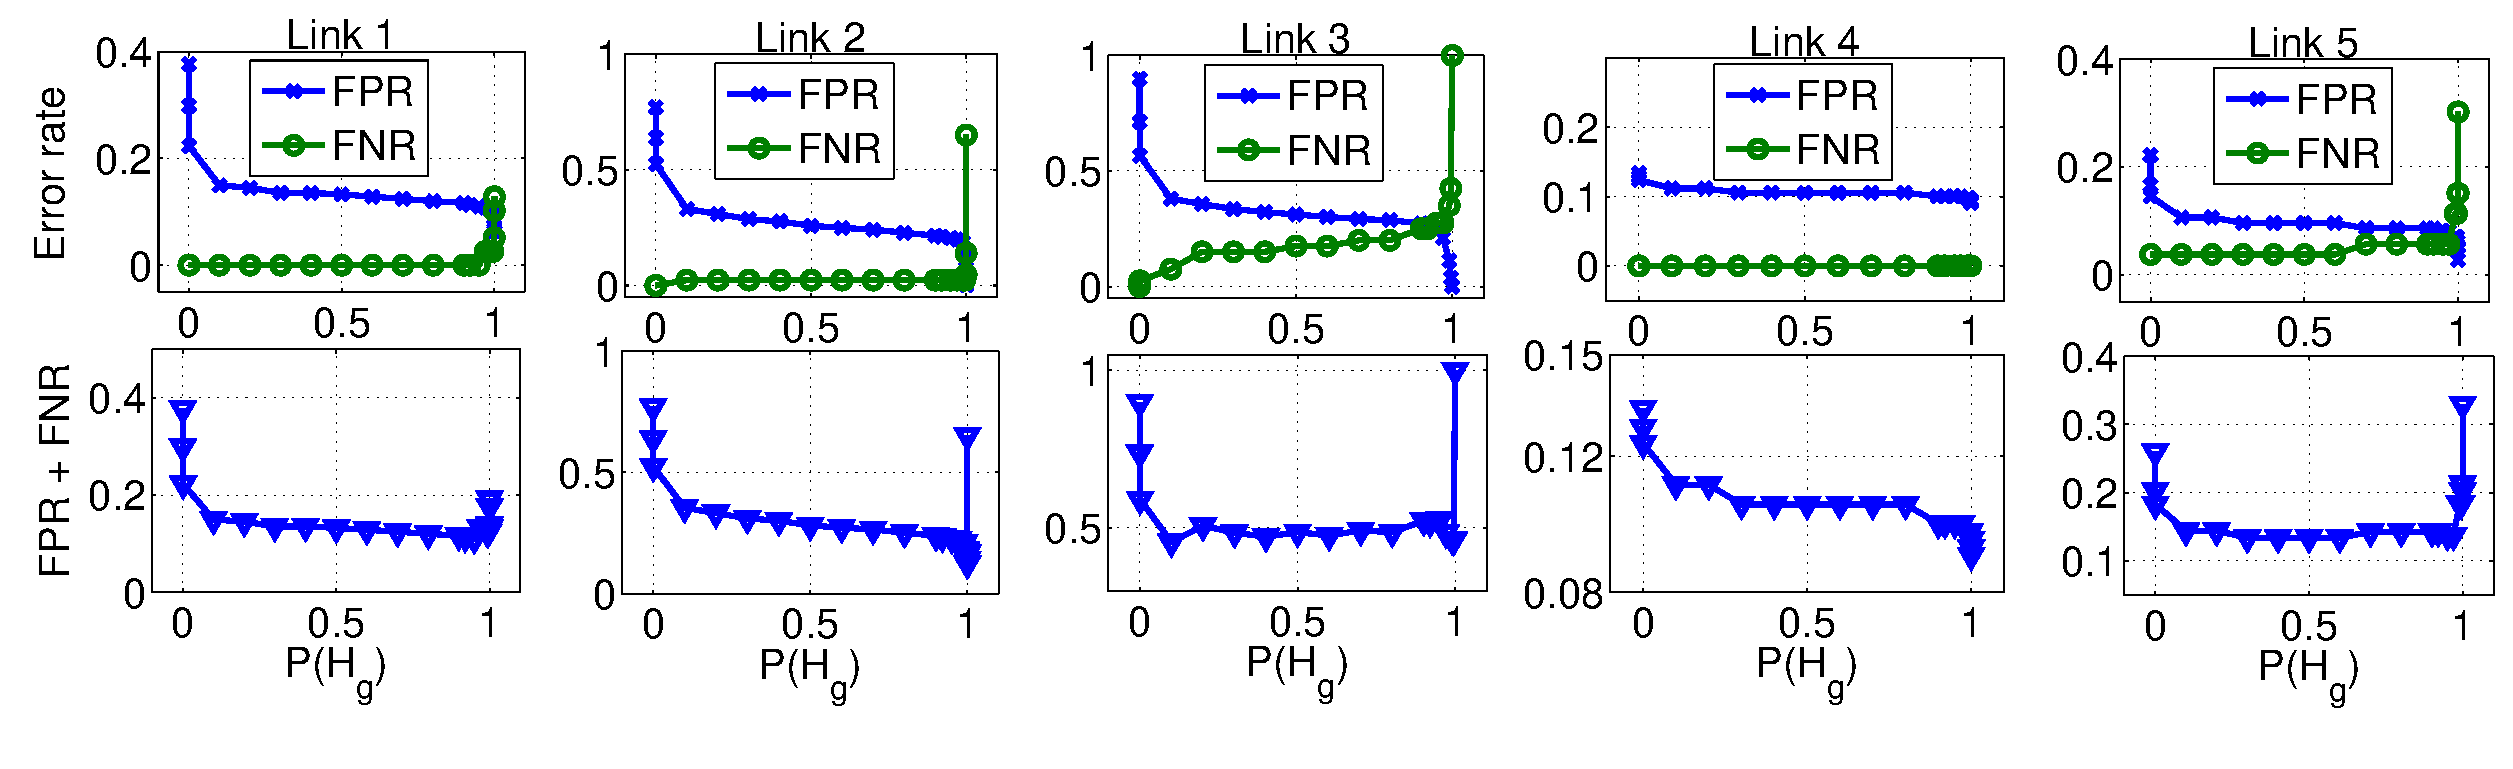
\includegraphics[width=1.0\linewidth, height = 5cm]{4-Find_ProbGood3}
	\vspace{-1.1cm}
	\caption{\textbf{Effect of the \textit{a priori} probability $P(H_g)$ on the error rates for 5 representative links. $P(H_g)$ varies in the range [$10^{-5}$, $1-10^{-5}$].} }
	\label{fig:EVA-ProbGood}
	\vspace{-0.4cm}
\end{figure*}
	
	
	
\begin{figure*}[t]
	\centering
	\begin{minipage}{.35\textwidth}
		\centering
		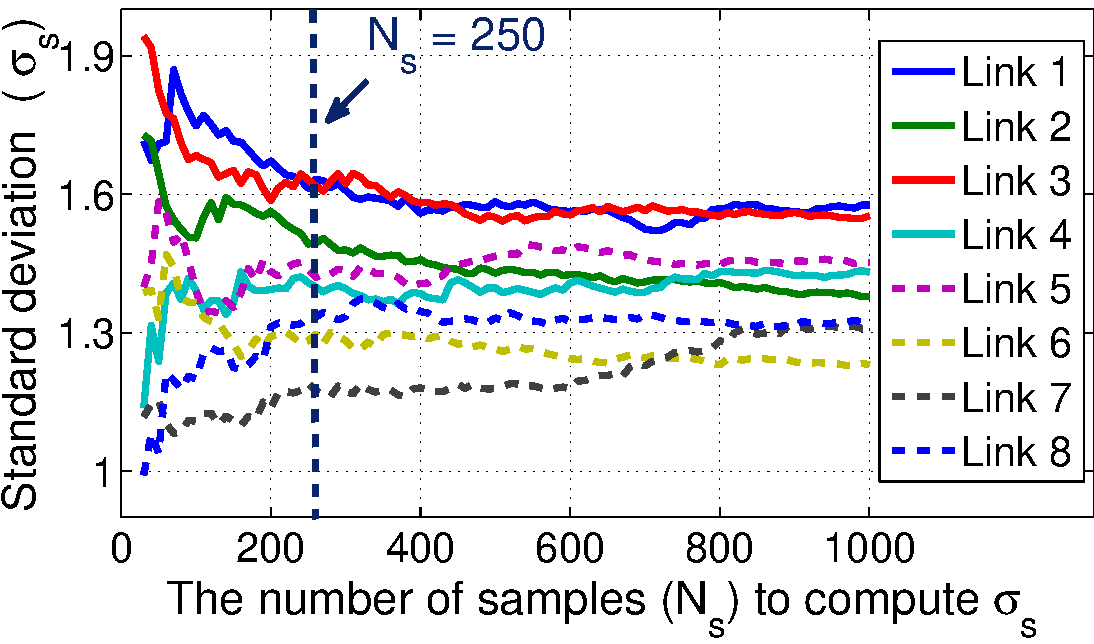
\includegraphics[width=1\linewidth, height=4cm]{1-Find_N_sigma3}
		\vspace{-0.75cm}
		\captionof{figure}{\textbf{Effect of the parameter $N_s$. The resultant $\sigma_s$ becomes more stable after $N_s = 250$.} }
		\vspace{-0.5cm}
		\label{fig:Nsigma}
	\end{minipage} \hfill
	\begin{minipage}{.6\textwidth}
		\centering
		%\vspace{-0.5cm}
		%\includegraphics[width=1\linewidth, height=4cm]{fig/2-Find_MeanError2}
		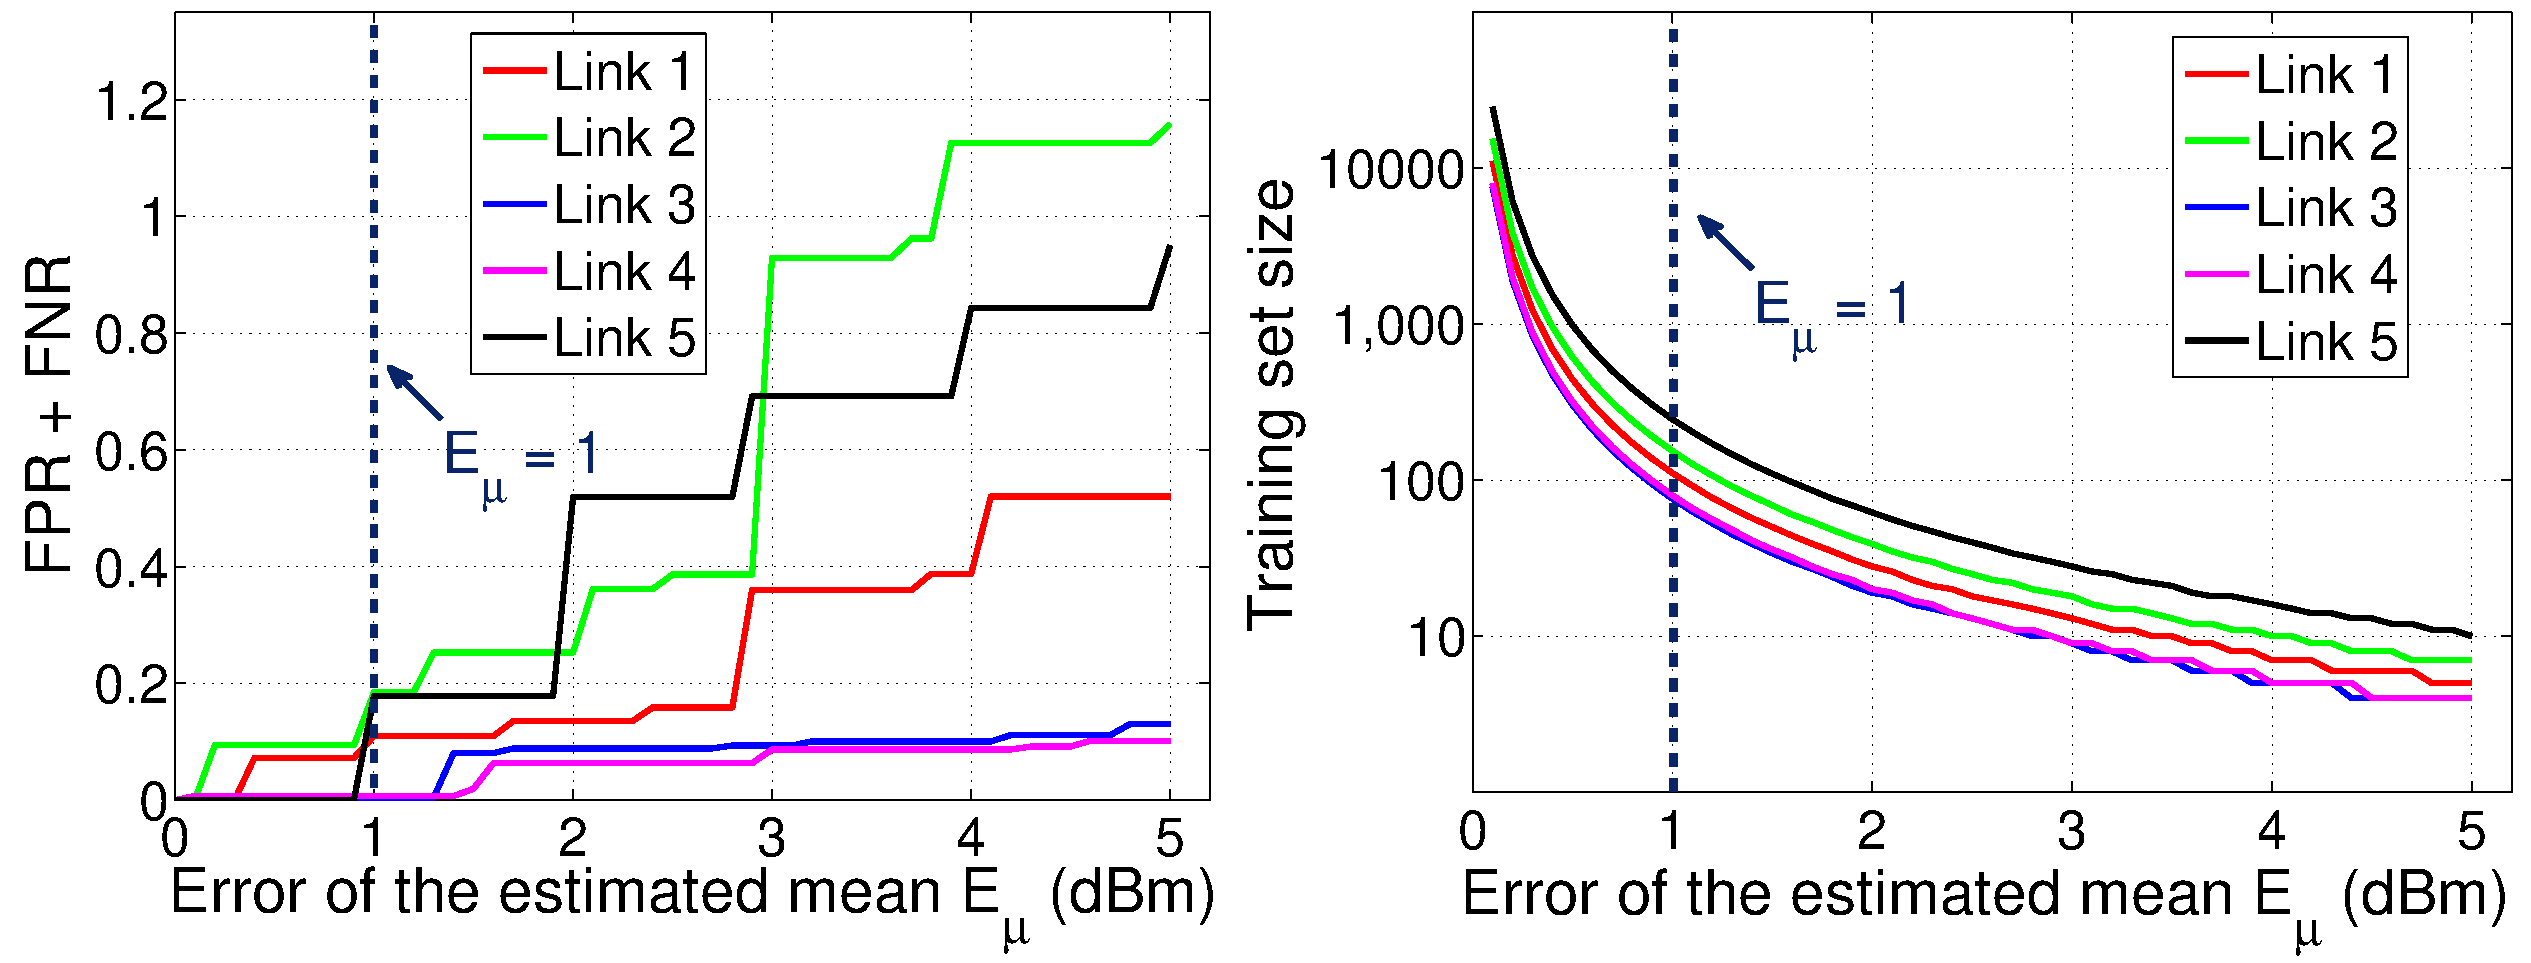
\includegraphics[width=1\linewidth, height=4cm]{2-Find_MeanError4}
		\vspace{-0.75cm}
		\captionof{figure}{\textbf{Effect of the parameter $E_{\mu}$. $E_{\mu} = 1$ dBm provides a good tradeoff between the detection accuracy and the training set size (i.e. training latency).}}
		\vspace{-0.5cm}
		\label{fig:ErrorMean}
	\end{minipage}
\end{figure*}

In the previous section, we presented the details of the Bayesian thresholding and the supporting techniques in RADIUS. We now study the impact of the aforementioned parameters required in each individual technique on the system performance. Specifically, we elaborate the effect of the Bayes threshold parameter $P(H_g)$ and then explore the parameter space of all the parameters involved in supporting techniques. Based on detailed analysis, we give insights on the best parameter setting for an indoor office environment.

For this, we performed extensive experiments, collecting real data traces from an indoor testbed, whose details are reported in Section \ref{sec:evaluation}. To capture different link conditions, we selected 8 sender-receiver pairs (either line-of-sight or non-line-of-sight) at different locations with various environment dynamics (e.g., human movements and obstacles). In each experiment, we simulated a good link turning into a weak link by decreasing the transmission power of the sender node from the maximum level gradually to the minimum with a packet sending rate of 5 Hz. The receiver node records the RSSI and PDR traces for more than 15 minutes. We repeated the experiment 10 times for each link. The minimum PDR that decides whether a link is a good link or a weak link is set to 80\% throughout the whole analysis.



\subsection{Bayesian Thresholding} \label{sec:ThresholdChoice}

According to Equation \ref{equ:rssiTHD}, calculating the Bayes threshold
%only 
requires a user-defined parameter: \textit{a priori} probability $P(H_g)$.
%if the underlying conditional distribution of the RSSI values is known from the training RSSI samples. 
Different from the general analysis depicted in Section \ref{sec:motivationBayes}, we present here the detailed analysis of the impacts of $P(H_g)$ on the false positive rate (FPR), false negative rate (FNR) and the total error rate. 
 
Figure \ref{fig:EVA-ProbGood} shows the change of the error rates with varying $P(H_g)$ ranging in [$10^{-5}$, $1-10^{-5}$] for 5 representative links out of the 8 analyzed links. We observe that the FPR always decreases with $P(H_g)$, while the FNR increases with $P(H_g)$. This is because a larger $P(H_g)$ indicates a higher weight on the FPR in the computation of the Bayes error (see Equation \ref{equ:error}). Hence,  reducing FPR is more effective than reducing FNR to keep the Bayes error rate low for a larger $P(H_g)$.  

Moreover, we can see in Figure \ref{fig:EVA-ProbGood} that the overall error rate mostly stays low regardless of the values of $P(H_g)$, except for the cases when the value of $P(H_g)$ is extremely close to 0 or 1. The results confirm that the system performance with the Bayes threshold is insensitive to the setting of $P(H_g)$ as long as extreme values are not considered. The reason for this is that the Bayesian thresholding approach always tries to balance between FPR and FNR for any $P(H_g)$ setting. 

From the figure, we can further see that a global $P(H_g)$ setting from a wide range (any value not close to 0 or 1) may not be the best setting for each individual link. However, it can provide for all different links near optimal detection accuracy at the same time. In other words, with a coarse global setting of $P(H_g)$ for all DAs, the Bayesian thresholding ensures RADIUS to deliver near optimal accuracy for different links under diverse link conditions without the need of tuning for each of them. For our case, we select the initial setting of $P(H_g)$ at 0.8 because we assume that the probability of the links being good is generally higher than that of being weak, in our deployment environment. Additionally, to avoid the significant increase of FNR caused by the over-adjustment due to the \textit{a priori} probability refinement, we limit the \textit{maximum} $P(H_g)$ to 0.99 for our deployment environment.




\subsection{Estimating the Minimal Training Set Size}\label{sec:evaParamTrainingSize}

As discussed in Section \ref{sec:minTrainingSet}, the first task of a DA before generating a Bayes threshold is to estimate the minimal training set size $N_{ts}$ for each link. A proper $N_{ts}$ needs to achieve a good tradeoff between detection accuracy and training latency. To apply Equation \ref{equ:minSampleSize}, the computation of $N_{ts}$ requires two parameters: (1) the number of first $N_s$ samples of RSSI for computing the standard deviation $\sigma_s$, and (2) the maximum error of the estimated mean  $E_{\mu}$. While the first $N_{s}$ samples of RSSI only give a quick indication, $N_{ts}$ is the resultant minimal training set size, from which the DA estimates the RSSI mean and standard deviation for computing Bayes thresholds. $N_{ts}$ is usually larger or at least equal to $N_{s}$.   

We first study the impact of $N_{s}$. A small $N_{s}$ may result in a partial view of the complete channel variation, while overly large $N_{s}$ may only increase the training delay. To understand the impact of $N_{s}$, we plot in Figure \ref{fig:Nsigma} the resultant standard deviation $\sigma_s$ for various values of $N_s$ based on the RSSI traces of all 8 links. We observe that the values of $\sigma_s$ initially have a larger variation and become more stable when $N_s$ is close to 250. The reason for this is that a small set of samples is insufficient to capture the overall temporal variations of RSSI, especially in an indoor environment where multi-path fading and interference are ubiquitous. Based on the result, we choose $N_s = 250$ for our indoor environment. %we conclude that, to find a good approximation of $\sigma_p$, we need to find the minimum value for $N_s$ with a converged $\sigma_s$, e.g., we select $N_s = 250$.
  
Then we focus on the impact of $E_{\mu}$. According to Equation \ref{equ:minSampleSize}, the choice of $E_{\mu}$ has a tradeoff: smaller $E_{\mu}$ indicates higher estimation accuracy of the RSSI mean and thus higher detection accuracy; a smaller $E_{\mu}$, however, may also increase the training set size significantly. By varying the estimated errors $E_{\mu}$, we plot the resultant training set size and error rates for 5 representative links in Figure \ref{fig:ErrorMean}. 
%For each link, we use the mean of 2000 samples in the RSSI trace as the true mean (we believe that 2000 samples are enough to give a nearly-true population mean for our environment, i.e., $E_{\mu} = 0$ dBm).  
The figure shows that the total error rate decreases significantly with a smaller $E_{\mu}$ at the expense of a rapidly increasing training set size. To balance between the detection error and the training time, we choose $E_{\mu} = 1$ dBm for our indoor environment, which causes only a slight increase of the detection error compared to that of $E_{\mu} = 0$ dBm while at the same time keeping $N_{ts}$ within the scale of a few hundred samples, achieving a good tradeoff between the training latency (several minutes with a sending frequency of 5 Hz) and detection accuracy. 

\begin{figure}[t]
	\centering
	%\vspace{-0.6cm}
	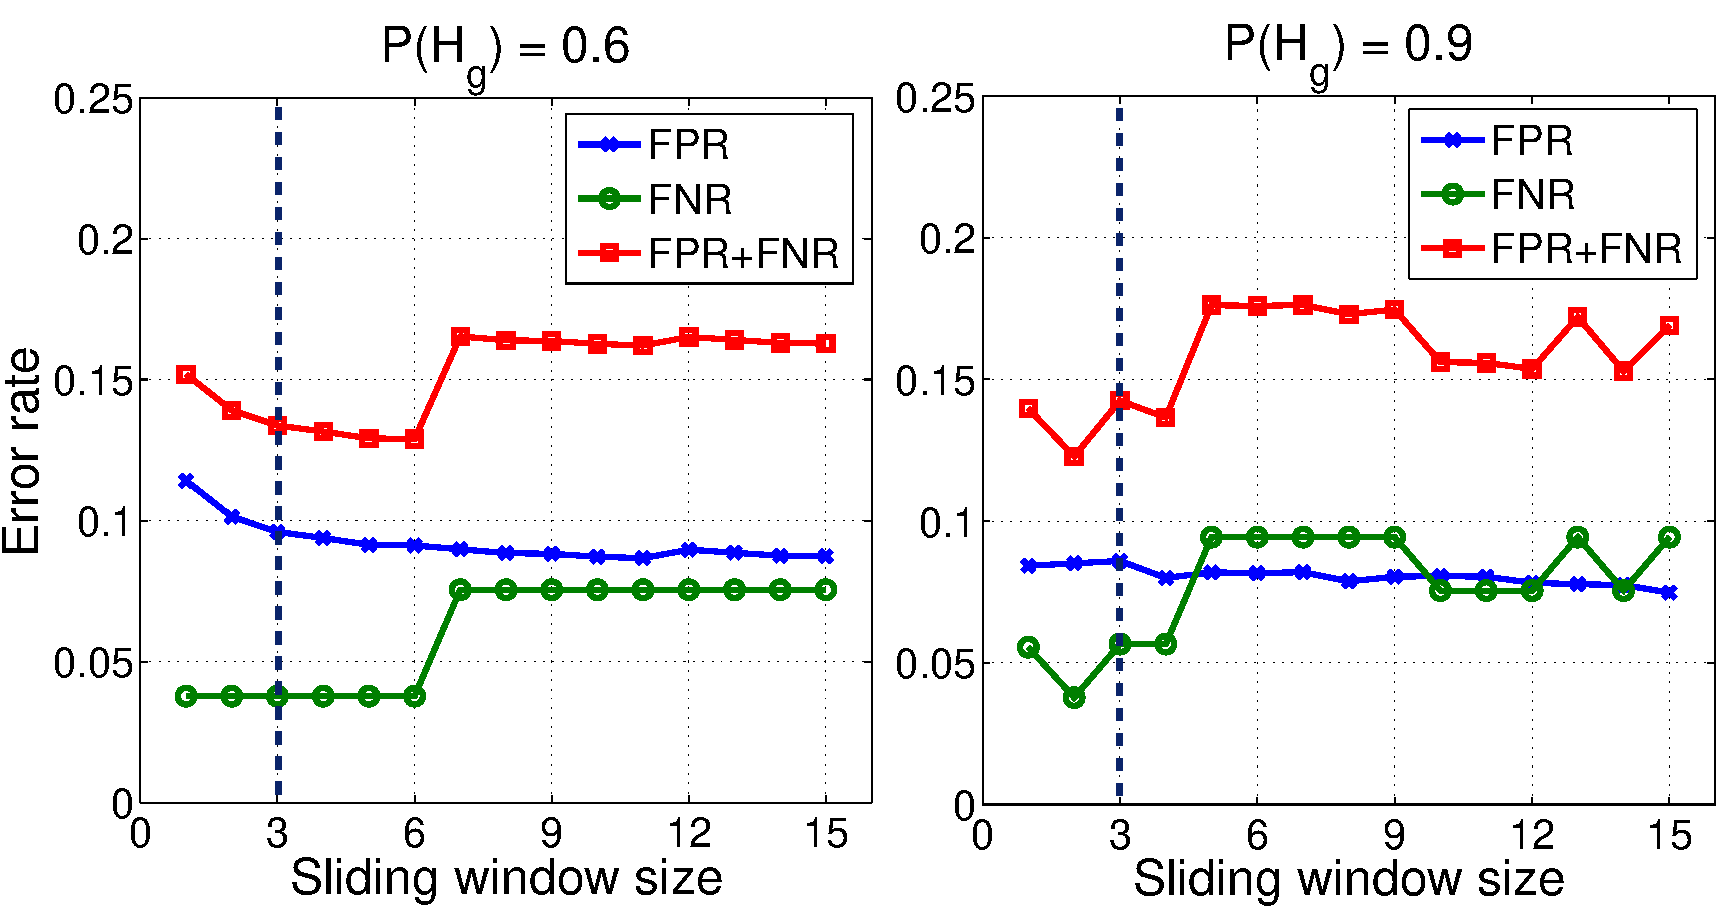
\includegraphics[width=1.0\linewidth, height = 4.5cm ]{3-Find_SlidingWindowSize_5}
	\vspace{-0.7cm}
	%\caption{Effect of data smoothing with different sliding window size $l$ for different $P(H_g)$. Error rate is close to lowest when $l = 3$ in all cases. }
	\caption{\textbf{Effect of data smoothing with different sliding window size $l$ for different $P(H_g)$. Error rate is close to lowest when $l=3$.} }
	%\caption{Effect of the sliding window size $l$ for different $P(H_g)$. As $l$ increases, FPR decreases while FNR increases. We choose $l = 3$.}
	\label{fig:EVA-slidingWindow}
	\vspace{-0.3cm}
\end{figure} 

\begin{figure}[t]
	\centering
	\includegraphics[width=1.0\linewidth, height = 6cm]{6-Find_UpdateWindowSize-WithPerson-nonLoS-UpDownUpDown-L1R1-2}
	\vspace{-1cm}
	\caption{\textbf{Effect of training set (TS) update with varying update window size $l_{update}$.}}
	\label{fig:EVA-updateWindow}
	\vspace{-0.7cm}
\end{figure} 

\subsection{Data Smoothing} \label{sec:ImpactDataSmoothing}

As mentioned in Section \ref{sec:dataSmoothing}, smoothing the noisy data during the detection phase requires a sliding window of size $l$ to reduce the detection error caused by the normal RSSI randomness. To see the impact of $l$, we demonstrate how the error rate changes with different values of $l$ (window size from 1 to 15) under two representative $P(H_g)$ values.

We observe from Figure~\ref{fig:EVA-slidingWindow} that, for both $P(H_g)$ settings, increasing $l$ reduces FPR but increases FNR, which causes the total error rate to first decrease and then increase with a larger $l$. The reason is that smoothing RSSI is effective to reduce false alarms. However, if $l$ keeps increasing, at some point, the real RSSI anomaly events are smoothed out, causing a significant increase in FNR. The impact of $l$ is also related to the setting of the minimal PDR ($PDR_{min}$) that defines a good link. In our case, as PDR is computed over a sliding window of 10 packets and $PDR_{min}$ is set to 80\%, a small sliding window $l$ is preferred to avoid the significant increase in FNR. For our case, we choose $l = 3$, at which the total error rate is close to the lowest for both $P(H_g)$ settings.  



\begin{figure}[t]
	\centering
	%\includegraphics[width=1.0\linewidth, height = 8cm]{fig/7-Find_AlarmNum_and_AdjustStep-WithPerson-nonLoS-L1R3-makeup2}
	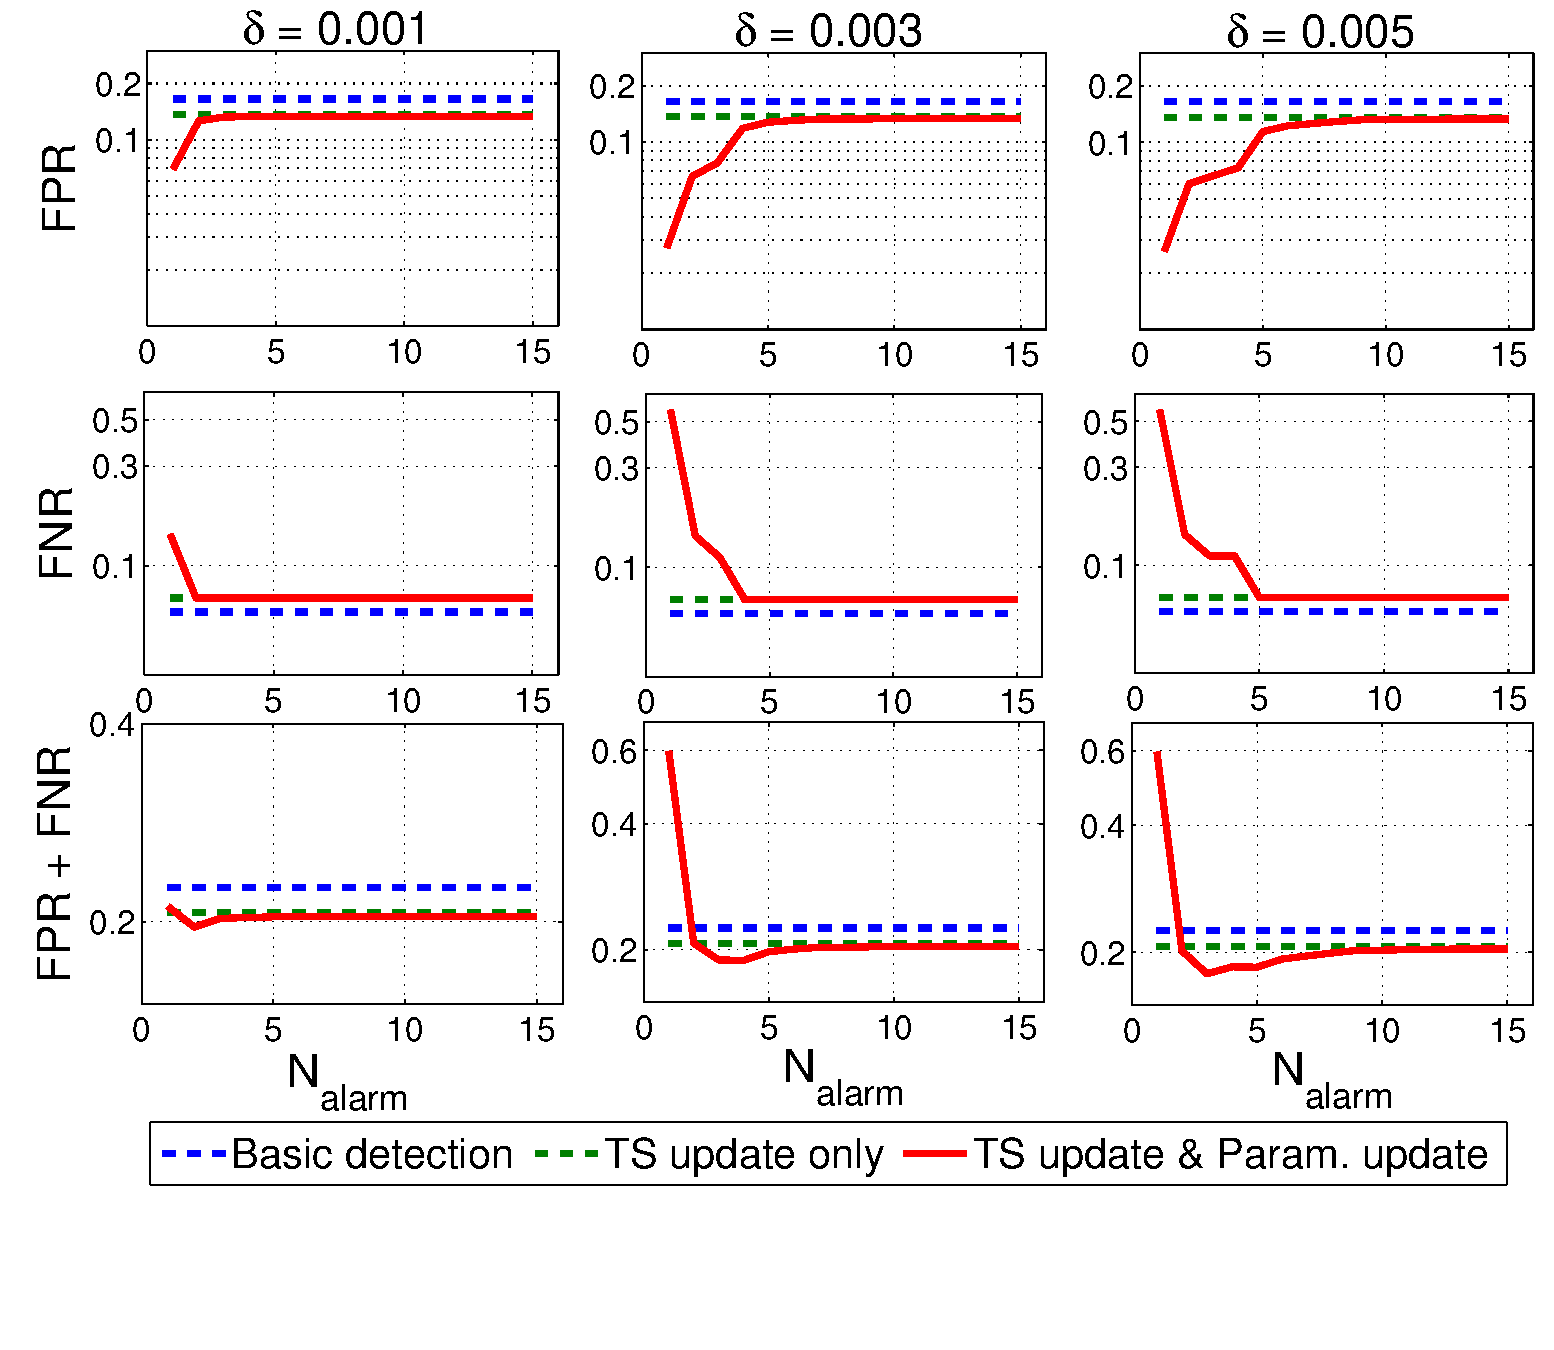
\includegraphics[width=1.0\linewidth, height = 8cm]{7-Find_AlarmNum_and_AdjustStep-WithPerson-nonLoS-L1R3-makeup2-v2}
	\vspace{-1.5cm}
	\caption{\textbf{Effect of the \textit{a priori} refinement with varying $N_{alarm}$ and $\delta$.}}
	\label{fig:EVA-paramRefine}
	\vspace{-0.65cm}
\end{figure}

\subsection{Updating the Training Set} \label{sec:evaParamTrainingUpdate}

To be adaptive to varying environment conditions, RADIUS updates the training set as discussed in Section \ref{sec:trainingSetUpdate}, dynamically generating new thresholds. For this, the relevant parameter is the update window size $l_{update}$. We first show that the detection performance is enhanced with this updating technique, and then we discuss the impact of $l_{update}$.

In Figure~\ref{fig:EVA-updateWindow}(a), we present an RSSI trace with a valley of RSSI values (between 300 and 500 seconds) indicating an abnormal situation that causes the monitored PDR to fall below the expected performance as shown in Figure~\ref{fig:EVA-updateWindow}(b). By adapting the training set and consequently the threshold (see Figure~\ref{fig:EVA-updateWindow}(c)), we can see from Figure~\ref{fig:EVA-updateWindow}(d) that in this experiment, the detection error can be reduced of 3\%-4\% with updated thresholds, down from 18\% to 14\% approximately.

%\begin{figure}[t]
%	\centering
%	\includegraphics[width=1.0\linewidth, height = 7cm]{fig/6-Find_UpdateWindowSize-WithPerson-nonLoS-UpDownUpDown-L1R1-2}
%	\vspace{-1.1cm}
%	\caption{Effect of training set (TS) update with varying update window size $l_{update}$.}
%	\label{fig:EVA-updateWindow}
%	\vspace{-0.5cm}
%\end{figure} 


Furthermore, we also observe from Figure~\ref{fig:EVA-updateWindow}(d) that the impact of $l_{update}$ is not significant on the detection error
%, and therefore the parameter choice is more tolerate 
(we set $l_{update}$ to be 50 for our example deployment). However, a larger $l_{update}$ may require a longer time to fill up the window making the threshold update less responsive in some cases. With such setting of $l_{update}$, we observe the detection error can be reduced of 3\% to 8\% in all experiments. Considering that the total error rate in most of our experiments is less than 20\%, such amount of reduction in the error rate is significant. 






\subsection{Refinement of the A Priori Probability}\label{sec:EVA-paramRefine}


In addition to updating the training data set, one other situation that requires to generate a new threshold is when the detection accuracy degrades with an increasing number of false alarms, indicating the need of updating the \textit{a priori} probability. As described in Section \ref{sec:prioriRefinement}, we consider the maximum number of consecutive false alarms $N_{alarm}$ and the adjustment step $\delta$ of $P(H_g)$. We quantify the effects of these parameters in Figure \ref{fig:EVA-paramRefine}, where we compare the detection accuracy with and without the refinement of the \textit{a priori} probability. Specifically, we show the detection performance with varying $N_{alarm}$ and $\delta$. We use the suggested values in the above sections for the other parameters.

%\begin{figure}[t]
%	\centering
%	\includegraphics[width=1.0\linewidth, height = 8cm]{fig/7-Find_AlarmNum_and_AdjustStep-WithPerson-nonLoS-L1R3-makeup2}
%	\vspace{-1.1cm}
%	\caption{Effect of the \textit{a priori} probability refinement with varying $N_{alarm}$ and $\delta$.}
%	\label{fig:EVA-paramRefine}
%	\vspace{-0.8cm}
%\end{figure}


From Figure \ref{fig:EVA-paramRefine}, we can see that a smaller $N_{alarm}$ can reduce FPR but it may also cause a significant increase in FNR due to over-adjustment. On the other hand, a larger $N_{alarm}$ makes the system conservative on the \textit{a priori} probability refinement and hence the refinement less effective. The optimal choice of  $N_{alarm}$ falls at the location where the total error rate is lowest. In addition, the choice of the parameter $\delta$ needs to consider a tradeoff: larger $\delta$ indicates a more effective adjustment but a higher risk of over-adjustment. In our example, we choose $N_{alarm} = 5$ and $\delta = 0.003$. With such parameter settings, the analysis of all data traces shows that based on the accuracy improvement achieved by the training set updating technique, refining $P(H_g)$  can further reduce the error rate in a range from 2\% to 5\%. 
% on the basis of applying the training set update.  




